\chapter{Introduction}
\section{C$_4$ Photosynthesis \& C$_4$ rice}

\begin{wrapfigure}{r}{0.5\textwidth}%
	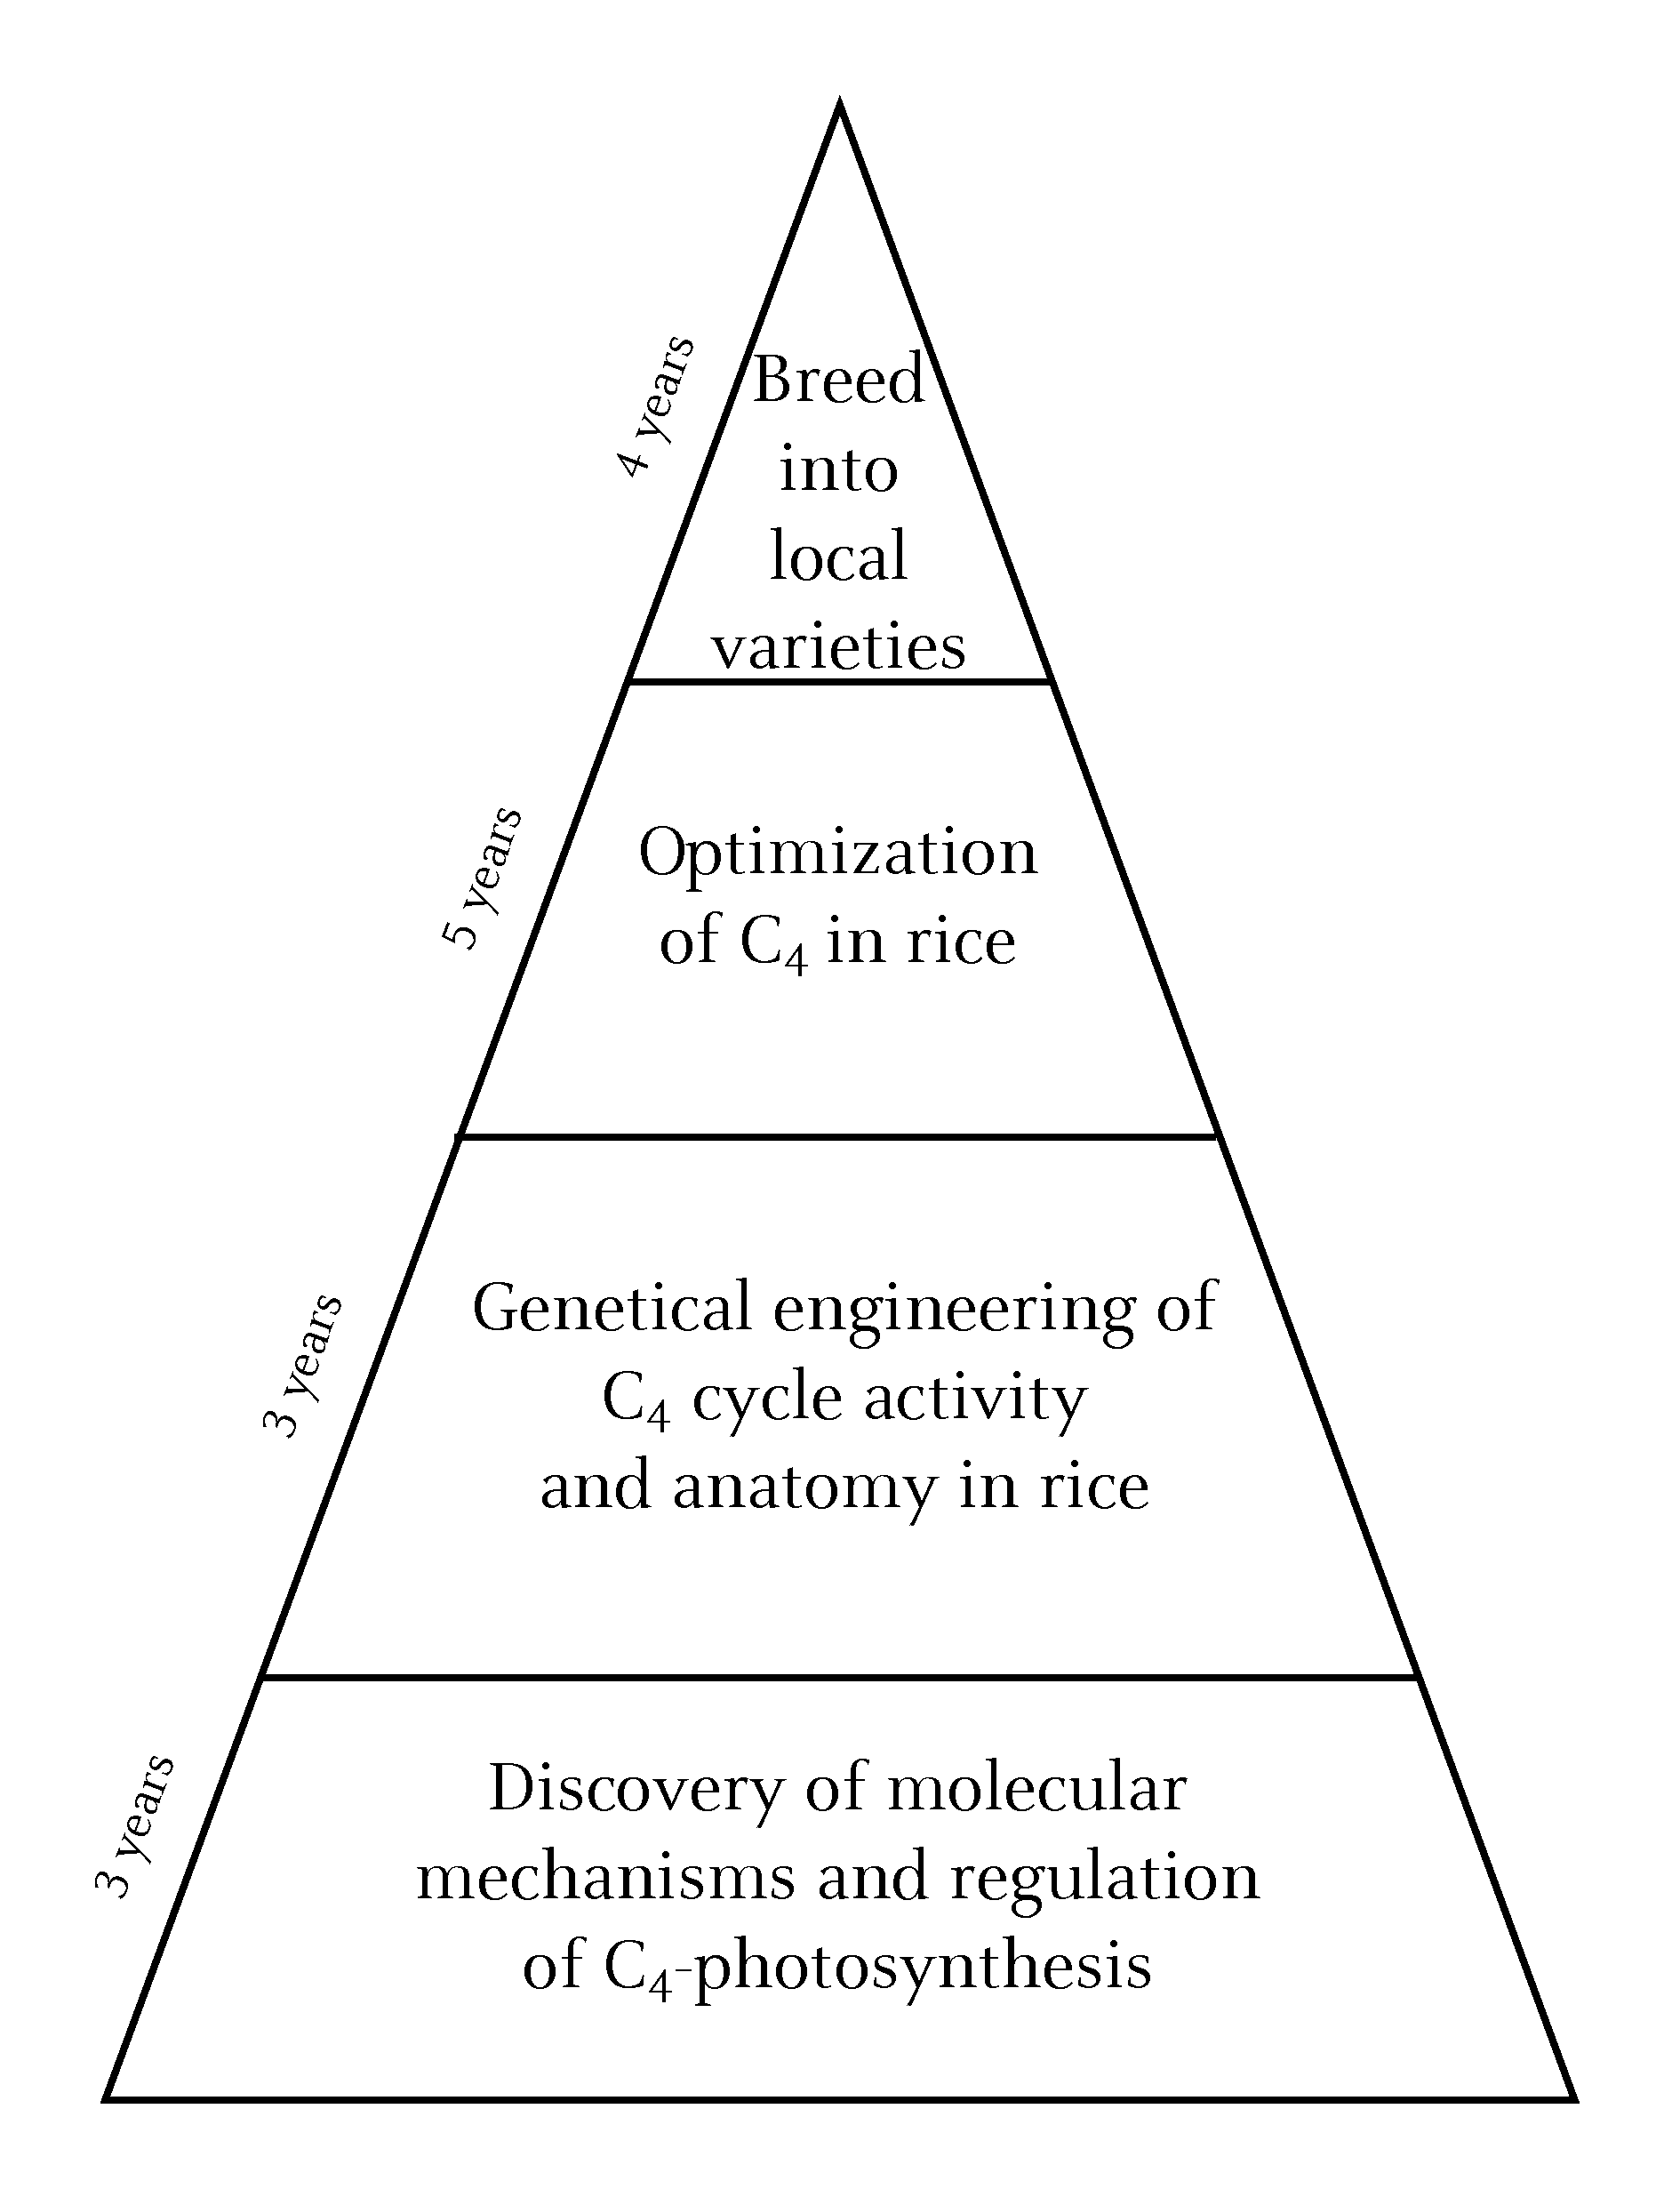
\includegraphics[width=0.48\textwidth]{images/C4_roadmap}%
	\caption{Roadmap for the C4-Rice Project \href{http://c4rice.irri.org}{(c4rice.irri.org)}}%
	\label{fig:c4rice_roadmap}%
\end{wrapfigure}

Around one billion people in the world feed on rice.
Rice is a cheap, non-perishable crop.
However, with growing population sizes the demand for rice increases, as well.
Now, C4 photosynthesis is considered a very promising trait to cope with this demand.
C4 photosynthesis is a trait that has evolved independently over 60 times throughout the plant kingdom.
Within the \species{Poaceae} (grasses) the evolutionary origins of C4 photosynthesis are confined within the PACMAD clade.
Plants performing C4 photosynthesis are avoiding energy loss by photorespiration.



%NOTES
Things I need to answer:
\begin{itemize}
	\item What is characteristic of C4-photosynthesis
	\item Why is it important to investigate
	\item What is the research goal
\end{itemize}
\section{Next-Generation Sequencing}
\section{Motivation}
